% Crucial Preamble
\documentclass[12pt,letterpaper]{article} \usepackage{amsmath} \usepackage{graphicx} \usepackage[margin=1in]{geometry} \usepackage{longtable}  \usepackage{amssymb}

% Extra Preamble
\usepackage{fancyhdr} \usepackage{enumitem} \usepackage{float} \usepackage{soul}
\usepackage{multicol} \usepackage[compact]{titlesec} \usepackage{listings}


% frames with display breaks
\usepackage{mdframed}
\allowdisplaybreaks

% change spacing
\usepackage{setspace}
\setlength{\parskip}{0.4\baselineskip}

% Remove paragraph indentation
\setlength{\parindent}{0pt}

% Reduce space before and after section headings
%\titlespacing*{\section}{0pt}{0.1\baselineskip}{0.2\baselineskip}

% changes font
%\renewcommand{\familydefault}{\sfdefault}

% adds header and footer
\pagestyle{fancy}
\fancyhead{} \fancyhead[C]{SEG 2106 Summary Sheet} \fancyhead[L]{SEG2106} \fancyhead[R]{Owen Daigle}
\fancyfoot{} \fancyfoot[C]{\thepage}

\definecolor{mygreen}{rgb}{0,0.6,0}
\definecolor{mygray}{rgb}{0.5,0.5,0.5}
\definecolor{mymauve}{rgb}{0.58,0,0.82}

\lstset{ %
	backgroundcolor=\color{white},   % choose the background color
	basicstyle=\footnotesize,        % size of fonts used for the code
	breaklines=true,                 % automatic line breaking only at whitespace
	captionpos=b,                    % sets the caption-position to bottom
	commentstyle=\color{mygreen},    % comment style
	escapeinside={<@}{@>},			 % Escapes these chars
	keywordstyle=\color{blue},       % keyword style
	stringstyle=\color{mymauve},     % string literal style
}


\begin{document}
	
	\begin{center}
		\Large\textbf{SEG 2106 Summary Sheet} \\
		\vspace{0.5em}
	\end{center}
	
	\section {Software Development Processes}
	\subsection{Black and White Box}
	The \textbf{black box} process gets the requirements for a project, then the team works on the project for a set period of time, and produces a product. 
	
	Thie \textbf{white box} process is similar to the black box process except for the stakeholders periodically check up on the project to provide \textbf{feedback}. 
	
	\subsection{Models}
	The \textbf{waterfall model} sequentially does domain analysis, gets requirements, makes a design, then tests and finally deploys. 
	
	This is very easy and good under ideal circumstances, but in the real word this is rarely used since \textbf{circumstances are rarely ideal}. Often stakeholders do not effectively communicate requirements to developers, or the requirements change. 
	
	We can modify the waterfall by adding \textbf{feedback} into the loop at each stage, so if we need to change something, we do not have to redo the whole project. This is an \textbf{agile development process}. 
	
	\section{Requirements Modeling}
	To get the requirements for a project, we need to analyse the domain the software will be used in. We need to understand the domain that the users are in so we can create software that works for the users. 
	
	We can make UML class diagrams for a system and all its parts. 
	
	\subsection{Requirements}
	We need to interview the stakeholders to figure out what they want. These are usually lots of sentences that say in general non technical terms what the system needs to do. 
	
	A system will have lots of use cases. Each use case is a "thing" that the user wants to do. Such as "create text file" or "delete file".
	
	We can create a use case diagram which is a diagram depicting all the use cases, and what user does that use case. 
	
	For each use case, we have the following information:
	\begin{itemize}[noitemsep]
		\item Actors
		\item Summary
		\item Precondition (does the system have to be in a specific state to do this use case?)
		\item Main Sequence (Sequence of what the user does and how the system responds)
		\item Alternative Sequences (Basically modifications to the main sequence depending on other events.)
		\item Postcondition (What state the system is in after the use case. )
	\end{itemize}

	\begin{mdframed}
		\textbf{Ex. } 
		% put example of use case diagram
	\end{mdframed}

	\textbf{Functional Requirements} are things that the system is supposed to do. 
	
	\textbf{Non Functional Requirements} are more about how the system is supposed to do something. Such as the system "must complete action in less than 5 seconds" or the system "must store password as encrypted".
	
	A \textbf{user story} is a more general form of a use case.
 	
	\section{Behavioral Modeling}
	
	\subsection{UML Activity Diagrams}
	This is a diagram that models behaviour of a system. They are good to model concurrent behaviour. 
	
	\begin{mdframed}
		\textbf{Ex. } 
		% put ex of activity
	\end{mdframed}
	
	\subsection{UML State Machines}
	This is a high level diagram that models the states of a certain part of a system. It is good at working with a single object/part. 
	
	\subsection{Petri Nets}
	This is a diagram that is good for modeling complex concurrent behaviour. They get very complex very fast though, so they are not great for large projects unless we have a large time budget. 
	
	A petri net works off of tokens. Tokens can trigger transitions that will cause tokens to move locations, add new tokens, or consume tokens. 
	
	A petri net is \textbf{bounded} if the number of tokens cannot exceed a finite amount. Conversely, a petri net is \textbf{unbounded} if \textit{there exists at least one} way for a petri net to create an infinite number of tokens. 
	
	A petri net is \textbf{alive} if there is always at \textit{least one transition } that can be fired from any point. Conversely, if there is any reachable combination where the system cannot do anything else (it dies), the petri net is not alive. 
	
	\begin{mdframed}
		\textbf{Ex. }
		% put ex of petri with boundedness and aliveness calculation
	\end{mdframed}
	
	\subsection{Specification and Description Language (SDL)}
	SDL has 3 main hierarchical levels. System, Block, and Process. 
	
	A system has one or more blocks interconnected with other. 
	
	A process is a state machine that has states and transitions, kind of like a UML state machine. 
	
	\section{Lexical Analysis}
	This is one part of a compiler. It checks that all the words in the program are \textbf{part of the language. }
	
	For example, if the language is java, "print" is not a word, but "if" and "System.out" are words. 
	
	Regular Expressions are used to do this. 
	
	\subsection{Alphabet}
	The \textbf{alphabet} are all the characters that we are working with. If a letter not in the alphabet is found, then the string is not accepted. 
	
	\begin{mdframed}
		\textbf{Ex. } If the alphabet is {a,b,c} then:
		
		"aaa" may be good
		
		"aaabbbbcccc" may be good
		
		"aaabbbcccddd" is NOT good since "d" is not in the alphabet. 
		
	\end{mdframed}

	\subsection{Operations}
	Union is the or operator. A|B means A or B
	
	Concatenation is 2 consecutive strings. AB means the string AB, not BA, AA, BB...
	
	Kleene Closure is the set of all strings that can be created from 0 or more strings defined. (aa)* means kleene closure of (aa) which is "", "aa", "aaaa", "aaaaaa", but not "a", "ab", "aaa"...
	
	Positive closure is like kleene closure but excludes the empty string. So, (aa)+ is the positive closure of (aa) which is "aa", "aaaa", ... Note the exclusion of "".
	
	\subsection{NFA}
	Non-deterministic Finite Automata (NFA) are a type of machine that model a regular expression. These have multiple states that are connected to each other with transitions. These transitions can be either $\epsilon$ (the empty string) or any value in the alphabet. 
	
	We use the following rules to convert a regular expression (regex) into an NFA:
	\begin{center}
		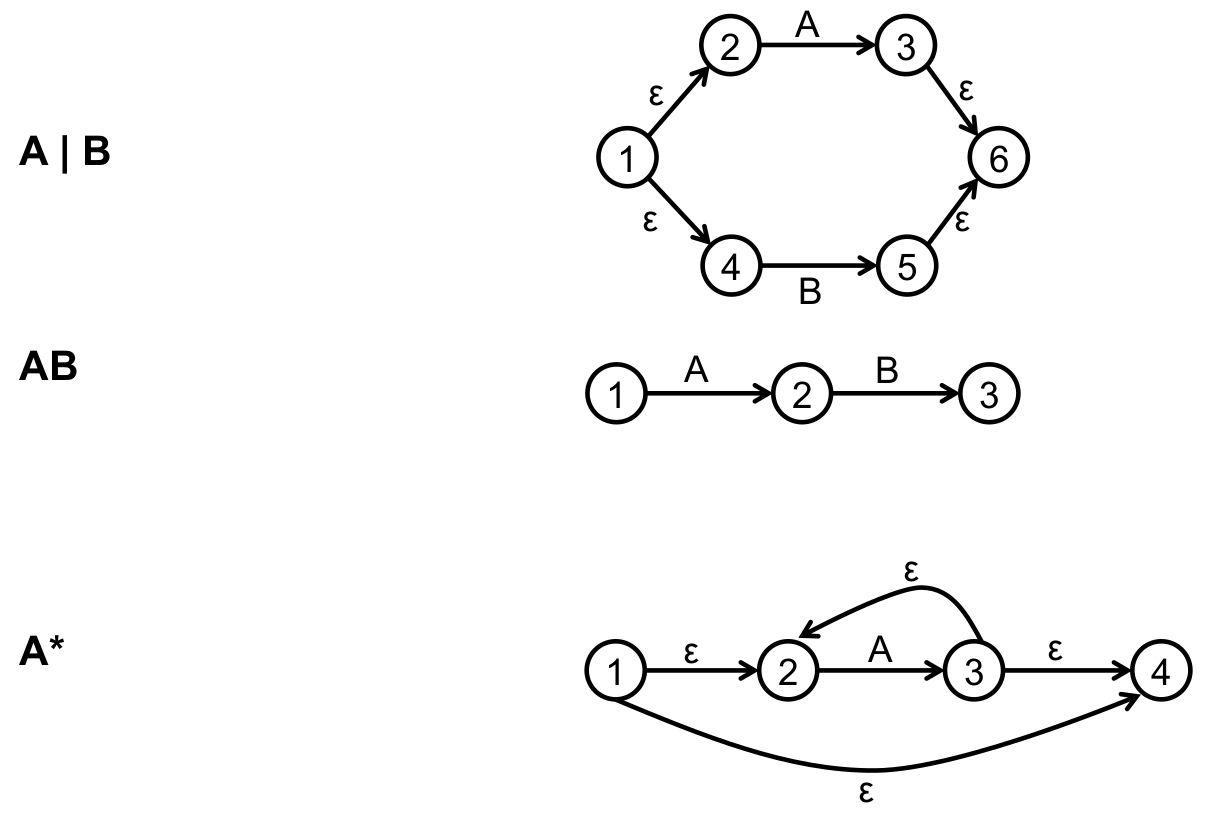
\includegraphics[width=0.7\linewidth]{nfa-rules}
	\end{center}

	We can combine these together to model more complicated REGEX such as (a|b)* which is just the A* design, but instead of A, we substitute the A|B design.
	
	\begin{mdframed}
		\textbf{Ex. } Find the NFA of \_\_\_\_\_
		% fill in later
	\end{mdframed}
	
	\subsection{DFA}
	NFA is easy to get, but it is hard for the computer to interpret it. This is where the Deterministic Finite Automata (DFA) comes into play. We create this using the \textbf{subset construction algorithm} on a NFA. In worst case scenario, we could have $2^n$ states where $n$ is the number of states in NFA.
	
	We have 2 functions.
	
	$\epsilon$-closure(S) is the state of the system that is reached by all epsilon transitions from state S. 
	
	move(S,a) will be the state the system is in after starting in state S and then taking the transition a.
	
	Basically, we make a table with all the states of the system (up to $2^n$) as rows, and colums for each letter of the alphabet. Then we perform move for each row (S), and each column (a)
	
	\begin{mdframed}
		\textbf{Ex. } Get the DFA of the following NFA through the subset construction algorithm:
		% fill in later
	\end{mdframed}
	
	\section{Syntax Analysis}
	% for later
	The parser is the part that takes in the tokens from scanner and checks that the grammar is correct. 
	
	We work with Context Free Grammars (CFG). 
	
	A CFG contains: 
	\begin{itemize}
		\item Terminals - Tokens produced by lexical analyser (actual raw code we are working with)
		\item Non terminals - Variables that denote sets of strings
		\item Start Symbol - A Special non terminal which is where we start
		\item Productions - Specify the manner the terminals and non terminals can be combined (Grammar Rules)
	\end{itemize}
	\begin{mdframed}
		\textbf{Ex.} This is an example of a grammar. 
		\begin{lstlisting}
<expr> ::= <expr> <op> <expr> | id | num
<op> ::= + | - | * | /	
		\end{lstlisting}
		We start with \verb*|<expr>| which can become either the terminals \verb*|id| or \verb*|num|, or can take on a non terminal of \verb*|<expr> <op> <expr>|.
		
		Then the \verb*|<op>| nonterminal can take on any of the operators. 
		
		Note that this grammar is useful for variable additions, subtractions, etc, such as:
		\begin{lstlisting}[language=java]
a + 1 // <expr> <op> <expr>
b - 5 // <expr> <op> <expr>
c * c + 1 // <expr> <op> (<expr> <op> <expr>)
		\end{lstlisting}
	\end{mdframed}
	\subsection{Parse Trees and Ambiguity}
	We can create a parse tree from a grammar to parse a certain string. 
	
	We call a grammar \textbf{ambiguous} if more than one parse tree can be created for a certain string. 
	
	\begin{mdframed}
		\textbf{Ex.} Using the previous grammar provided, produce a parse tree for \verb*|id+id*id|. 
		
		We start with the starting symbol. Then we need to expand one of the \verb*|<expr>| nonterminals to get \verb*|<expr><op><expr>|, then web sub in \verb*|id| for each \verb*|<expr>|, and the corresponding operators. 
		\begin{center}
			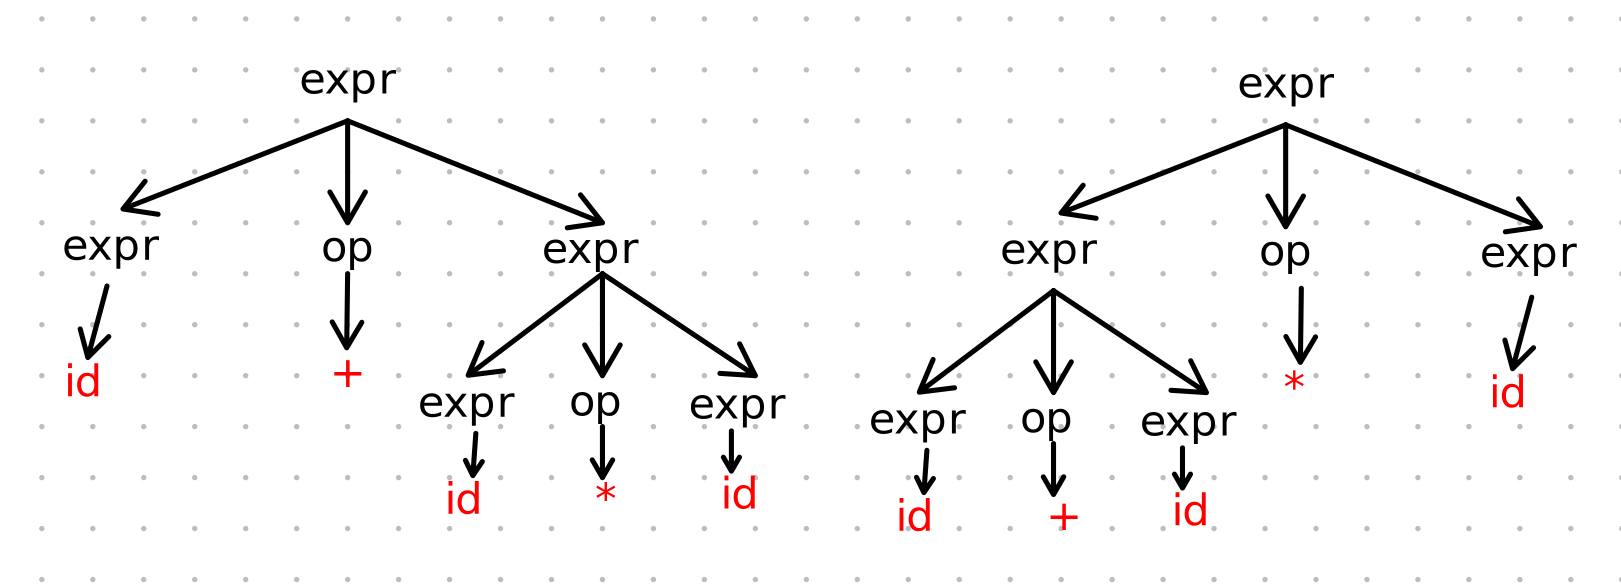
\includegraphics[width=0.7\linewidth]{2-parse-trees-ex}
		\end{center}
		We can actually create at least \textbf{two} parse trees for this same string. So we know that this grammar is ambiguous as well (uh oh).
	\end{mdframed}

	It is very hard to methodically eliminate ambiguity, and not something that is done in this course. 

	\subsection{Left Recursion}
	This is where there is a rule such as $A \implies A\alpha |\beta$ where $A$ is a nonterminal, and $\alpha$ is anything else. 
	
	This is a problem since the parser will expand $A$ to get $A\alpha$. Then it will expand that $A$ to get $A\alpha\alpha$. Then again to get $A\alpha\alpha\alpha$ and so on. It will get stuck in an infinite loop. 
	
	Whenever a rule like that exists, we need to remove it. 
	
	We fix this by doing:
	\begin{lstlisting}
A ::= bA'
A' ::= aA' | <@$\epsilon$@>
	\end{lstlisting}
	instead of:
	\begin{lstlisting}
A ::= Aa | b
	\end{lstlisting}
	
	\subsection{Left Factoring}
	If we have a grammar rule that says $A ::= Ba | Bc$, then we do not know where it should go. If we see a $B$, do we go to the first rule, or the second rule? 
	
	We can figure this out by backtracing if we choose the wrong rule, but this is inefficient. 
	
	To do this, we will change that rule into two rules of $A ::= BA'$, and $A' ::= a|b$.
	
	\subsection{FIRST and FOLLOW sets}
	These are two sets that need to be calculated for the computer to do syntax analysis. 
	
	Formally they are defined as:
	\begin{center}
		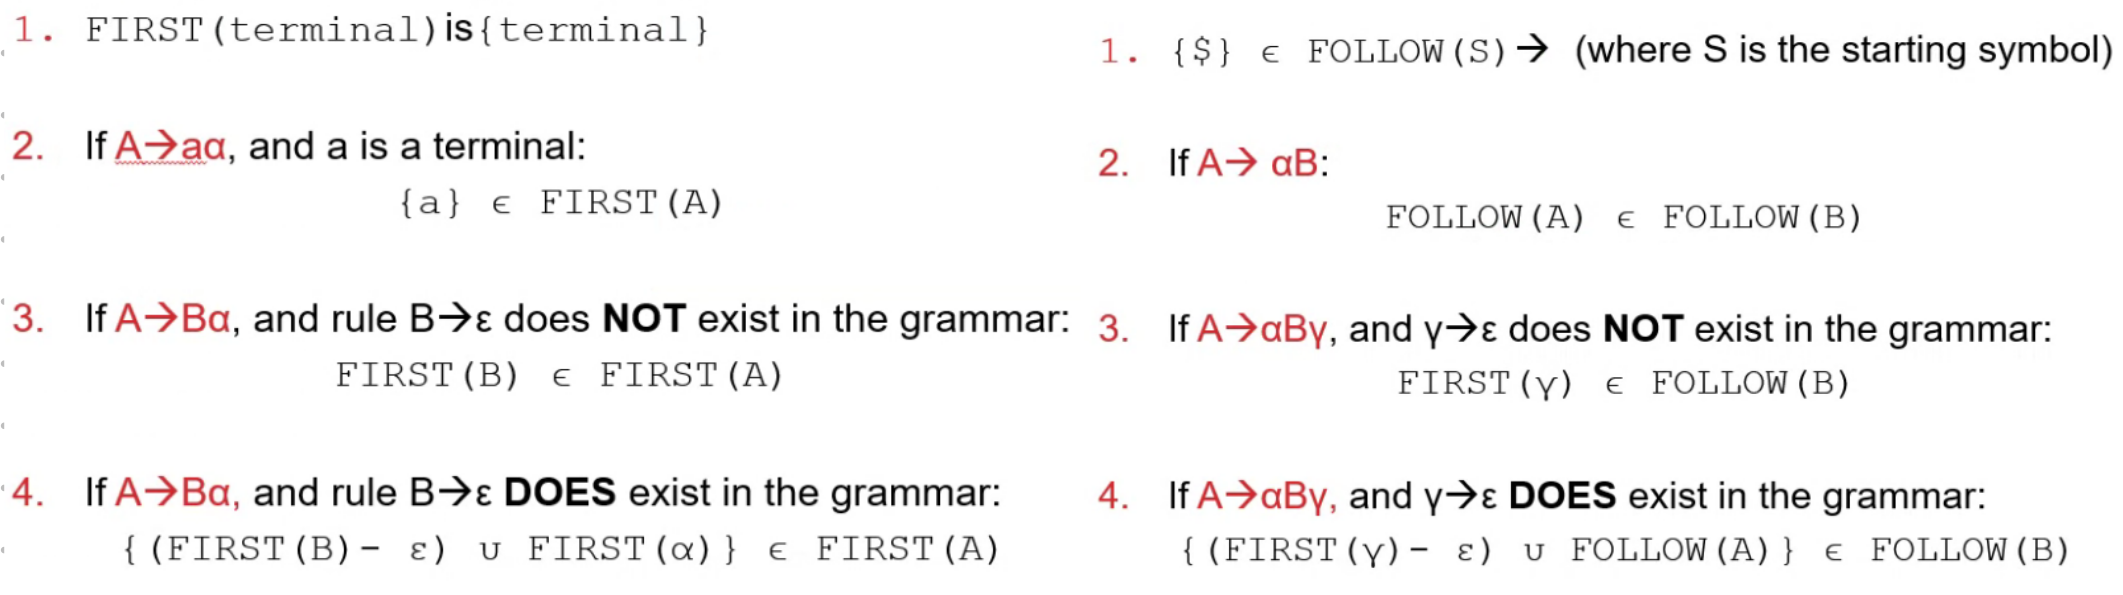
\includegraphics[width=0.9\linewidth]{first-follow-formal}
	\end{center}
	These definitions are a bit hard to follow though. 
	
	Informally, the FIRST set contains the FIRST of all the nonterminals. The FIRST of a nonterminal is the \textbf{first terminal that will show up} in place of this nonterminal. 
	
	Informally the FOLLOW set contains the FOLLOW of all the nonterminals. The FOLLOW of a nonterminal is the \textbf{first terminal that appears after} this nonterminal. 
	
	\begin{mdframed}
		\textbf{Ex.} Remove left factoring and left recursion from this grammar. Then create the first and follow sets. 
		\begin{lstlisting}
<program> ::= <@\texttt{\textcolor{blue}{\{<statement\_list>\} }}@>
<statement_list> ::= <@\texttt{\textcolor{blue}{<statement>;<statement\_list> }}@> | <@\texttt{\textcolor{blue}{<statement>; }}@> 
<statement> ::= <@\texttt{\textcolor{blue}{call: <procedure\_call> }}@> | <@\texttt{\textcolor{blue}{compute: <expression> }}@> 
<procedure_call>::= <@\texttt{\textcolor{blue}{id(<parameters>) }}@> 
<parameters>::= <@\texttt{\textcolor{blue}{<factor>,<parameters> }}@> | <@\texttt{\textcolor{blue}{<factor> }}@> 
<expression> ::= <@\texttt{\textcolor{blue}{id=<factor>+<factor> }}@> | <@\texttt{\textcolor{blue}{id=<factor>-<factor> }}@> | <@\texttt{\textcolor{blue}{id=<factor> }}@> 
<factor> ::= <@\texttt{\textcolor{blue}{id|num }}@> 
		\end{lstlisting}
		To remove \textbf{left recursion}, we need to look for something like $A::=A\alpha$. We do not have anything of the sort present. 
		
		To remove \textbf{left factoring}, we look for where a rule can derive more than 1 rule each with the same first item. 
		
		This is the case with \verb*|<statement_list>| since both derivations start with \verb*|<statement>|. Following the rules for removing left factoring we get:
		\begin{lstlisting}
<statement_list> ::= <statement>;<statement_prime> 
<statement_prime> ::= <statement_list> | <@$\epsilon$@>
		\end{lstlisting}
		We also need to do this with \verb*|<parameters>| and \verb*|<expression>| to get:
		\begin{lstlisting}
<program> ::= <@\texttt{\textcolor{blue}{\{<statement\_list>\} }}@>
<statement_list> ::= <@\texttt{\textcolor{blue}{<statement>;<statement\_list'>}}@> 
<statement_list'> ::=<@\texttt{\textcolor{blue}{<statement\_list>}}@> | <@\texttt{\textcolor{blue}{$\epsilon$}}@> 
<statement> ::= <@\texttt{\textcolor{blue}{call: <procedure\_call> }}@> | <@\texttt{\textcolor{blue}{compute: <expression> }}@> 
<procedure_call>::= <@\texttt{\textcolor{blue}{id(<parameters>) }}@> 
<parameters> ::= <@\texttt{\textcolor{blue}{<factor><parameters'>}}@> 
<parameters'> ::= <@\texttt{\textcolor{blue}{,<parameters>}}@> | <@\texttt{\textcolor{blue}{$\epsilon$}}@>
<expression> ::= <@\texttt{\textcolor{blue}{id=<factor><expression'>}}@> 
<expression'> ::= <@\texttt{\textcolor{blue}{+<factor>}}@> | <@\texttt{\textcolor{blue}{-<factor>}}@> | <@\texttt{\textcolor{blue}{$\epsilon$}}@>
<factor> ::= <@\texttt{\textcolor{blue}{id|num }}@> 
		\end{lstlisting}
	
		Now to create the first set. 
		
		The FIRST for \verb*|<program>| would be just \verb*|{| since this is the first thing we see.
			
		The FIRST for \verb*|<statement_list>| is more complex. The first thing we see is the first of \verb*|<statement>| which is \verb*|call| or \verb*|compute|.
		
		We do this for each element. Now for the FOLLOW sets. 
		
		For \verb*|<program>| we see where \verb*|<program>| is found in the rules. It is never found. So the only thing that can come after it is the EOF (end of file) symbol \verb*|$|.
		
		For \verb*|<statement_list>|, we see that this is found in the definition of \verb*|<program>|, and \verb*|<statement_list'>|. 
		\begin{itemize}
			\item Considering the \verb*|<program>| rule, what follows is \verb*|}|. 
			\item Considering the \verb*|<statement_list'>|, well the last element is \verb*|<statement_list>|, so here we need to add the FOLLOW of \verb*|<statement_list>'| which is the FOLLOW of \verb*|<statement_list>| which means we can ignore this rule. 
		\end{itemize}
	
		So now we also have the FOLLOW of \verb*|<statement_list'>| which is also \verb|}|
	
		Then for \verb*|<statement>| the element following it is only \verb*|;|
		
		We end up getting:
		\begin{center}
			\begin{tabular}{|c|c|}
				\hline
				\begin{lstlisting}
FIRST(program) = {
FIRST(statement_list) = call compute
FIRST(statement_list') = call compute <@$\epsilon$@>
FIRST(statement) = call compute
FIRST(procedure_call) = id
FIRST(parameters) = id num
FIRST(parameters') = , <@$\epsilon$@>
FIRST(expression) = id
FIRST(expression') = + - <@$\epsilon$@>
FIRST(factor) = id num
				\end{lstlisting}&  
			\begin{lstlisting}
FOLLOW(program) = $
FOLLOW(statement_list) = }
FOLLOW(statement_list') = }
FOLLOW(statement) = ;
FOLLOW(procedure_call) = ;
FOLLOW(parameters) = )
FOLLOW(parameters') = )
FOLLOW(expression) = ;
FOLLOW(expression') = ;
FOLLOW(factor) = ; , + - )
			\end{lstlisting}\\
				\hline
			\end{tabular}
		\end{center}
	
	\end{mdframed}
	
	\subsection{Parse Tables}
	A Parse table is a table where the rows are all of the non terminals, and the columns are all the terminals including the end of line character $\$$.
	
	For the first row, we go through the FIRST set of that nonterminal. Each terminal that exists, we fill out that box with the rule associated to the nonterminal/terminal combination. 
	
	If the FIRST set contains the empty string $\epsilon$, then we also include the terminals from the FOLLOW set. 
	
	\begin{mdframed}
		\textbf{Ex.} For the previous example, the parse table is below:
		\begin{center}
			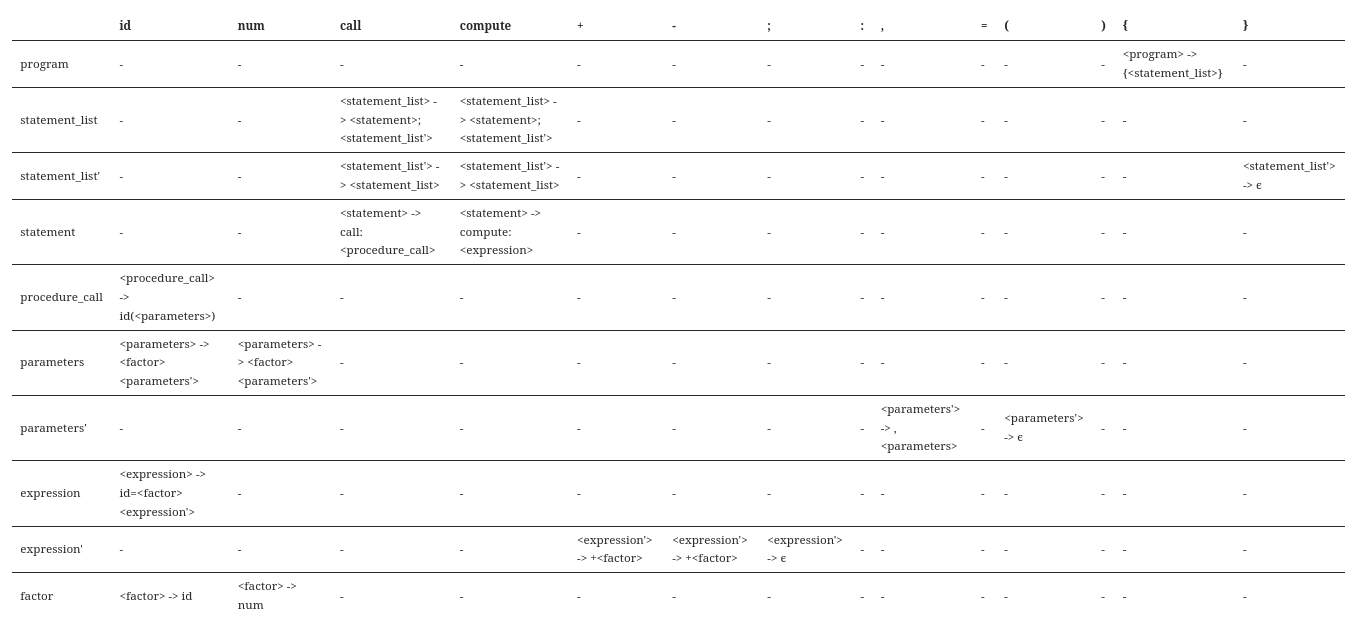
\includegraphics[width=1\linewidth]{ex-parsetable}
		\end{center}
		
	\end{mdframed}
	
	\subsection{LL1 Parsing}
	To actually do the LL1 Parsing, we make use of the \textbf{parse table. }
	
	We have a stack that we work with.
	\begin{enumerate}
		\item Push the \textbf{start symbol} onto the stack.
		\item Popping the top nonterminal on the stack, and the next terminal in the input stream, we then push the corresponding cell in the parse table.
		\item \textbf{IF} the top of the stack has a terminal, \textbf{THEN} we check if this terminal corresponds to the head of the input stream. 
		\subitem \textbf{IF YES} then we pop this element from the stack, as well as from the input stream and continue
		\subitem \textbf{IF NO then} the syntax does not follow the grammar and we have a problem. We \textbf{terminate the syntax analysis}
		\item \textbf{Return to step 2 and repeat} until no terminals left in the input stream.
	\end{enumerate}
	
	\subsection{Error Recovery}
	There can be two types of errors when parsing:
	\begin{enumerate}
		\item There is a missing token (like missing semicolen)
		\item There is an unexpected token (like extra semicolen)
	\end{enumerate}
	The parser will try to skip symbols from the input until it gets back in sync, then it will skip one from the stack. 
	
	We are in sync when the current cell is a cell in the follow set. 
	\begin{center}
		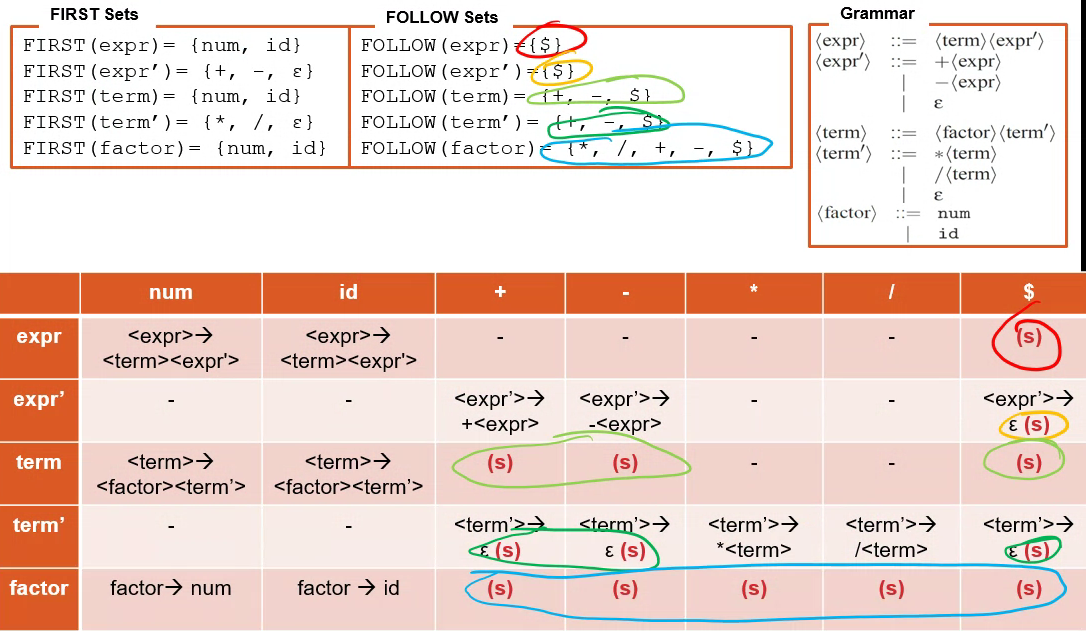
\includegraphics[width=1\linewidth]{sync-fromcoursenotes}
	\end{center}
	
	
	\section{Concurrency}
	% for later
	Concurrency means having \textbf{multiple threads} operating at the same time. It sounds simple, but it causes a lot of headaches. 
	
	The main problems are some methods only can be accessed by one thread at a time or it will cause problems. For example, if two threadas try to \textbf{write to a file at the same time},\textit{ which file do we keep}? That depends on who writes first. 
	
	For example, if two threads open a file that just has a counter variable inside (say at 0), and they each increment it by 1, and then both write the file, then depending on the order in which this was done, the counter variable in the file could either have value of 1, or 2. 
	
	This is known as \textbf{competition synchronization}.
	
	We also have \textbf{cooperation synchronization} which is where there is a shared resource that multiple tasks need access to such as a printer. Another good example is a producer/consumer example. If the consumer consumes faster than the producer produces, then it will need to wait a lot for the producer. 
	
	\subsection{Semaphores}
	A semaphore is a \textbf{counter}. This counter typically is either 1 or 0 (allowes access to only one thread) but could be more (such as allowing access to only up to 3 threads simultaneously). 
	
	For a thread to access the shared resource, it will need to \textbf{acquire} the semaphore with \verb*|wait(semaphore)| and when it is done it will \textbf{release} the semaphore with \verb*|release(semaphore)|.
	
	The \verb|wait| method will check if the semaphore's counter is greater than 0. If so, it will decrement the counter, and allow the task to access the resource. If the counter is 0, then it places the task in a queue.
	
	The \verb*|release| method will either increment the counter (if queue is empty) or dequeue the next task to have access to the resource. 
	
	\subsection{Deadlock}
	Deadlock happens when threads get to an impass and cannot proceed ever. 
	
	This often happens when a thread (Thread 1) requires another thread (Thread 2) to relenquish access to a resource. But Thread 2 is waiting for Thread 1 to relenquish access to a different resource. So neither can proceed. 
	
	This can be fixed by a few methods:
	\begin{itemize}
		\item Eliminating one of the semaphores. (Why not turn both semaphores into one semaphore)
		\item Recovering from deadlock by for example implementing time limits. (A semaphore gets auto released after 5 seconds or something)
	\end{itemize}
	
	\subsection{Monitors}
	A monitor is a set of routines that are protected by a mutual exclusion lock. 
	
	It is basically a very big semaphore that encompasses a lot of methods. 
	
	They are built in to the programming languages, so they are easy to implement and understand but they do not offer as much control as semaphores. 
	
	A monitor only allows \textbf{one task} to access \textbf{ANY} subroutines in the monitor at any given time. 
	
	Monitors have 2 methods. \verb*|wait(aQueue)| puts the current thread in a queue to get access to the monitor. \verb*|signal(aQueue)| tells the queue \verb*|aQueue| that it can let someone else into the monitor. 
	
	\subsection{Atomic Variables}
	An atomic variable is a variable that all modifications are done in a \textbf{single step}. This ensures synchronization. 
	
	They are a class such as \verb*|AtomicInteger| or \verb*|AtomicBoolean|.
	
	\subsection{Java Concurrency}
	A class can be made into a thread either by extending the \verb*|Thread| class, or implementing the \verb*|Runnable| interface. Both of these require the \verb*|public void run()| method to be implemented.
	
	A \verb*|ThreadGroup| is a container that holds multiple threads. It lets us stop all threads, or find out how many threads are currently running. 
	
	When threads are interrupted, they have a flag set to \verb*|true| and they throw an \verb*|InterruptedException|. 
	
	The \verb*|synchronized| keyword for a method means that that method can only have one thread executint that method at a time. If there are multiple \verb*|synchronized| methods in a class, only \textbf{one} can be executed at a given time. This is called an \textbf{intrinsic lock} (monitor).
	\begin{lstlisting}[language=java]
public synchronized int (getCount()) {
	counter++;
	return counter;
}
	\end{lstlisting}
	
	We can also use \verb*|synchronized| for a single block of code such as:
	\begin{lstlisting}[language=java]
synchronized (lock) {a = 1} //synchronized variable assignment using a lock

//this cannot execute while the previous line is executing since same lock
synchronized (lock) {a = 2} //also synchronized using the same lock 

synchronized (lock2) { //using a different lock
	b = 3
}
	\end{lstlisting}

	Cooperation synchronization is implemented using the \verb*|notify()| and \verb*|wait()| methods. These are used inside synchronized methods. 
	\begin{lstlisting}[language=java]
public synchronized int fetch() {
	while (buffer = 0) //while the buffer is empty
		wait();
	}
	//do some stuff 
	buffer--;
	notify(); //let someone else know that there is space in the buffer to add to
}
	\end{lstlisting}

	We can also use something like \verb*|reentrantLock()|. This gives us a lock that we can lock and unlock. When it is locked, no one else can unlock it. 
	
	\begin{lstlisting}[language=java]
public class ----- {
	private final Lock lock = new ReentrantLock(); //creates lock
	public void test() {
		lock.lock(); //now no one else can unlock the lock
		try{ /*do some stuff*/}
		finally {lock.unlock;} //we ALWAYS need to unlock or deadlock may occur
	}
}
	\end{lstlisting}

	We can also create conditions and use \verb*|condition.await()| to wait, and \verb*|condition.signal()| to signal threads waiting on that condition to wake up.

	
	
\end{document}